
%%%%%%%%%%%%%%%%%%%
%%% SVHN RESULTS
%%%%%%%%%%%%%%%%%%%


% \begin{figure}\CenterFloatBoxes
% \begin{floatrow}
% \ffigbox[1.0\linewidth][]{%
%     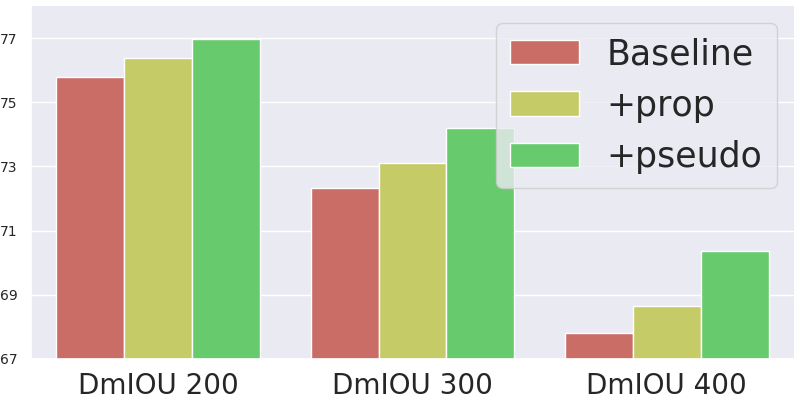
\includegraphics[height=0.4\linewidth]{figures/dmiou.png}
% }%
% {%
%     \vspace{-0.3em}%
%     \caption{\small Measuring the improvement on Distance based mIoU by training on pseudo-labels.}
%     \label{fig: figure-label}
% }%
% \killfloatstyle\ttabbox[\Xhsize]
% {%
%     \begin{tabular}[t]{llcc}
%         \toprule
%         \multicolumn{2}{l}{} & mIOU & $\text{\tiny DmIOU}_{200}$ \\
%         \midrule
%         \multicolumn{2}{l}{Baseline} &  &\\
%         \multicolumn{2}{l}{Baseline + SDC} & &\\
%         \multicolumn{2}{l}{Baseline + LID} & & \\
%         \multicolumn{2}{l}{Baseline + GT} & & \\
%         \bottomrule
%     \end{tabular}
% }%
% {%
%     \caption{\small Benefit of training with pseudo-labels on ApolloScape Dataset}\label{tab: table-label}
% }%
% \end{floatrow}

% % \caption{\small \emph{Left:} The sequence error for SVHN multi-digit recognition
% % on crops of $64\times 64$ pixels (64px), and inflated crops of $128 \times 128$
% % (128px) which include more background. \textsuperscript{*}The best reported
% % result from \cite{Ba14} uses model averagin}
% % % }}%
% \vspace{-1em}
% \end{figure}

\begin{table}[t]
    \centering
    \caption{ We show the benefit of training with our pseudo-labels. We also show the benefit of modelling label uncertainty. In the above table,  $D_{\hat{L}seq}$ contains propagated labels and $D_{\hat{L}ps}$ contains pseudo-semantic labels (refer Section~\ref{subsec-alea}).
    }\label{tab_main_ablation}
    \begin{tabular}{llcc}
\toprule
\multicolumn{2}{c}{Dataset}& Loss & mean IOU  \\
\midrule
\multicolumn{2}{l}{$D_L$} & C.E. & 77.62\\
\multicolumn{2}{l}{$D_L$ + \cite{nvidia_cvpr19} ($\pm 2,4,6,8$)}& RLL &77.82  \\
\multicolumn{2}{l}{$D_L$ + Ours ($\pm [2,4,6,8])$}&$\mathtt{UAT}$ & 78.45  \\
\midrule
\multicolumn{2}{l}{$D_L$ + GT($\pm [2,4,6,8])$}& \cite{gal_main} & 77.82  \\
\bottomrule
    \end{tabular}
\end{table}
 
% \begin{table}[t]
% \begin{center}\small
% % \setlength{\tabcolsep}{3pt}
% \begin{tabular}[t]{lccc}
% %%%%%% Title row starts here
% \\
% % Temporary header Graph would be better! TBD
% \toprule
% \multicolumn{1}{l}{} & $\text{{\tiny DmIOU}}_{200}$ & $\text{\tiny DmIOU}_{300}$ & $\text{\tiny DmIOU}_{200}$ \\
% \midrule
% \multicolumn{1}{l}{Baseline} & 75.79 & 72.32 & 67.80\\
% \multicolumn{1}{l}{+ prop} & 76.37 & 73.10 & 68.66 \\
% \midrule
% \multicolumn{1}{l}{+pseudo} & 76.37 & 73.10 & 68.66 \\
% \bottomrule
% \end{tabular}
% \qquad\qquad \qquad\qquad
% % \hspace{-2em}
% % \vtop{
% % \vspace{-1em}
% % \hbox{
% % 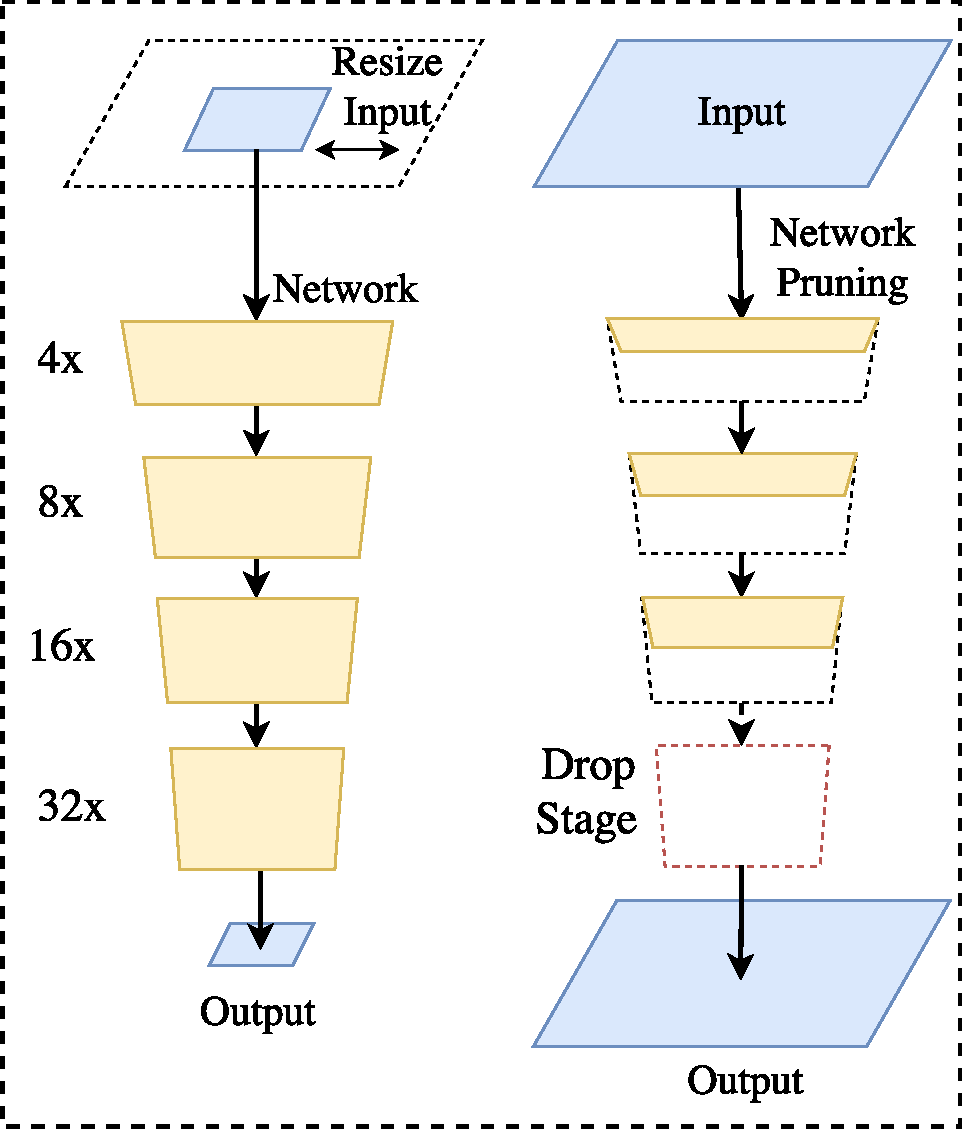
\includegraphics[width=0.6\textwidth]{figures/input_model.pdf}
% \begin{tabular}[t]{llcc}
% %%%%%% Title row starts here
% \toprule
% \multicolumn{2}{l}{} & mIOU & $\text{\tiny DmIOU}_{200}$ \\
% \midrule
% \multicolumn{2}{l}{Baseline} &  &\\
% \multicolumn{2}{l}{Baseline + SDC} & &\\
% \multicolumn{2}{l}{Baseline + LID} & & \\
% \multicolumn{2}{l}{Baseline + GT} & & \\
% \bottomrule
% \end{tabular}

% % }}%
% \end{center}
% \caption{\small \emph{Left:} The sequence error for SVHN multi-digit recognition
% on crops of $64\times 64$ pixels (64px), and inflated crops of $128 \times 128$
% (128px) which include more background. \textsuperscript{*}The best reported
% result from \cite{Ba14} uses model averagin}
% \label{table:svhn}
% \end{table}
